% Provenance (never printed): cycle 3 "La planete Terre" (natural phenomena
% and the risks they bring: storms, floods, droughts, earthquakes, eruptions;
% warnings and the right behaviour); see sources/book1/PROVENANCE.md.
% Book 1, grade 5, chapter 3.
\chapter{自然危害}\label{ch:g5:natural-hazards}

现在是星期五晚上。收音机里的音乐停了，一个平静的声音播报
了一则警报：今晚一场强\omterm{def:g5:natural-hazards:storm}{风暴}将抵达\omterm{def:g1:landscapes-around-us:water}{海岸}，风力很大，
并有暴雨。人们被要求从九点起待在室内，
把可能被风吹走的东西捆牢或搬进屋里。

莉娜一家立刻忙了起来。爸爸把花园里的椅子和
桌子搬进了小屋。妈妈检查手电筒能否使用，并把
备用电池放在厨房的桌子上。莉娜往两个大瓶子里
装满了水。九点时，大家都已进屋，外面的风已经
呼啸起来。

\begin{omfigure}

\includegraphics[width=0.5\linewidth]{images/book1/ai/g5-radio-warning.jpg}

{\small 一家人正在收听收音机里的\omterm{def:g5:natural-hazards:storm}{风暴}警报，
手电筒和备用电池已经准备好。}
\end{omfigure}

\begin{recall}
\omterm{def:g4:volcanoes-earthquakes-first-look:volcano}{火山}可能\omterm{def:g4:volcanoes-earthquakes-first-look:eruption}{喷发}，喷出\omterm{def:g4:volcanoes-earthquakes-first-look:eruption}{熔岩}、\omterm{def:g4:volcanoes-earthquakes-first-look:eruption}{火山灰}和气体；\omterm{def:g4:volcanoes-earthquakes-first-look:earthquake}{地震}是地面的
突然震动；遇到\omterm{def:g4:volcanoes-earthquakes-first-look:earthquake}{地震}时，要趴下、掩护并抓牢
（见\cref{ch:g4:volcanoes-earthquakes-first-look}）。当\omterm{def:g1:landscapes-around-us:water}{河流}接纳的水超过河道所能容纳的量时，
就会泛滥，淹没\omterm{def:g5:water-shapes-the-land:flood}{河漫滩}
（见\cref{ch:g5:water-shapes-the-land}）。每个地方都有自己的\omterm{def:g5:weather-and-climate:climate}{气候}，
炎热带、温带和寒带环绕着地球
（见\cref{ch:g5:weather-and-climate}）。
\end{recall}

\section{什么是自然危害}

大自然并不总是平静的。风可能强到足以吹倒
树木，\omterm{def:g1:landscapes-around-us:water}{河流}可能泛滥，大地可能震动。这些事件是
地球运行方式的一部分：它们早在有人类之前就已发生，
并且还会继续发生。

\begin{definition}[自然危害]\label{def:g5:natural-hazards:hazard}
\emph{自然危害}\index{自然危害}是指可能伤害人类或破坏人类所建造之物的
自然事件，例如\omterm{def:g5:natural-hazards:storm}{风暴}、\omterm{def:g5:water-shapes-the-land:flood}{洪水}、\omterm{def:g5:natural-hazards:drought}{干旱}、\omterm{def:g4:volcanoes-earthquakes-first-look:earthquake}{地震}、\omterm{def:g4:volcanoes-earthquakes-first-look:volcano}{火山}\omterm{def:g4:volcanoes-earthquakes-first-look:eruption}{喷发}、
\omterm{def:g5:natural-hazards:landslide}{滑坡}{\ldots}
\end{definition}

我们可以按\omterm{def:g5:natural-hazards:hazard}{自然危害}的来源进行分类：来自空气的、
来自水的，或来自地面的。

\begin{omfigure}
\begin{tikzpicture}[font=\small, box/.style={draw, rounded corners=3pt,
    minimum width=4.2cm, minimum height=0.9cm, align=center}]
  \node[box, fill=cyan!15, font=\small\bfseries] (A) at (0,0) {来自空气};
  \node[box, fill=blue!15, font=\small\bfseries] (W) at (4.8,0) {来自水};
  \node[box, fill=brown!25, font=\small\bfseries] (G) at (9.6,0) {来自地面};
  \node[align=center, anchor=north] at (0,-0.7) {风暴 \\热带气旋 \\热浪 \\干旱};
  \node[align=center, anchor=north] at (4.8,-0.7) {洪水 \\（来自河流、来自 \\暴雨、来自风暴中的 \\海水）};
  \node[align=center, anchor=north] at (9.6,-0.7) {地震 \\火山喷发 \\滑坡};
  \node[draw, rounded corners=3pt, fill=gray!10, font=\small\bfseries,
    minimum width=5cm, minimum height=0.8cm] (N) at (4.8,1.5) {自然危害};
  \draw[->] (N.south) -- (A.north);
  \draw[->] (N.south) -- (W.north);
  \draw[->] (N.south) -- (G.north);
\end{tikzpicture}

{\small 按来源分类的\omterm{def:g5:natural-hazards:hazard}{自然危害}。}
\end{omfigure}

\section{来自空气的危害}

\begin{definition}[风暴]\label{def:g5:natural-hazards:storm}
\emph{风暴}\index{风暴}是指风力非常强劲的\omterm{def:g1:watching-the-weather:weather}{天气}，通常伴有
暴雨或大雪，有时还伴有雷电。
\end{definition}

强\omterm{def:g5:natural-hazards:storm}{风暴}会折断树枝、刮倒树木、掀掉屋顶的瓦片，
还可能把花园里的椅子吹过窗户。在\omterm{def:g1:landscapes-around-us:water}{海岸}地区，风会把海水
推向岸边，并把巨浪卷过海堤。

地球上最强大的\omterm{def:g5:natural-hazards:storm}{风暴}形成于温暖的热带\omterm{def:g2:water-on-earth:ocean}{海洋}上方。它们是
巨大的旋转\omterm{def:g5:natural-hazards:storm}{风暴}：从太空看去，它们像一个巨大的云螺旋，
中间有一个平静、晴朗的空洞，称为\omterm{def:g5:natural-hazards:storm}{风暴}眼。\omterm{def:g5:natural-hazards:storm}{风暴}眼周围
吹着最强的风。同一种\omterm{def:g5:natural-hazards:storm}{风暴}在不同\omterm{def:g2:water-on-earth:ocean}{海洋}有不同的名称：
在北大西洋和东太平洋称为\emph{飓风}，
在西北太平洋称为\emph{台风}，
在南太平洋和印度洋称为\emph{热带气旋}。
% ledger: noaa:cyclone-names

\begin{omfigure}
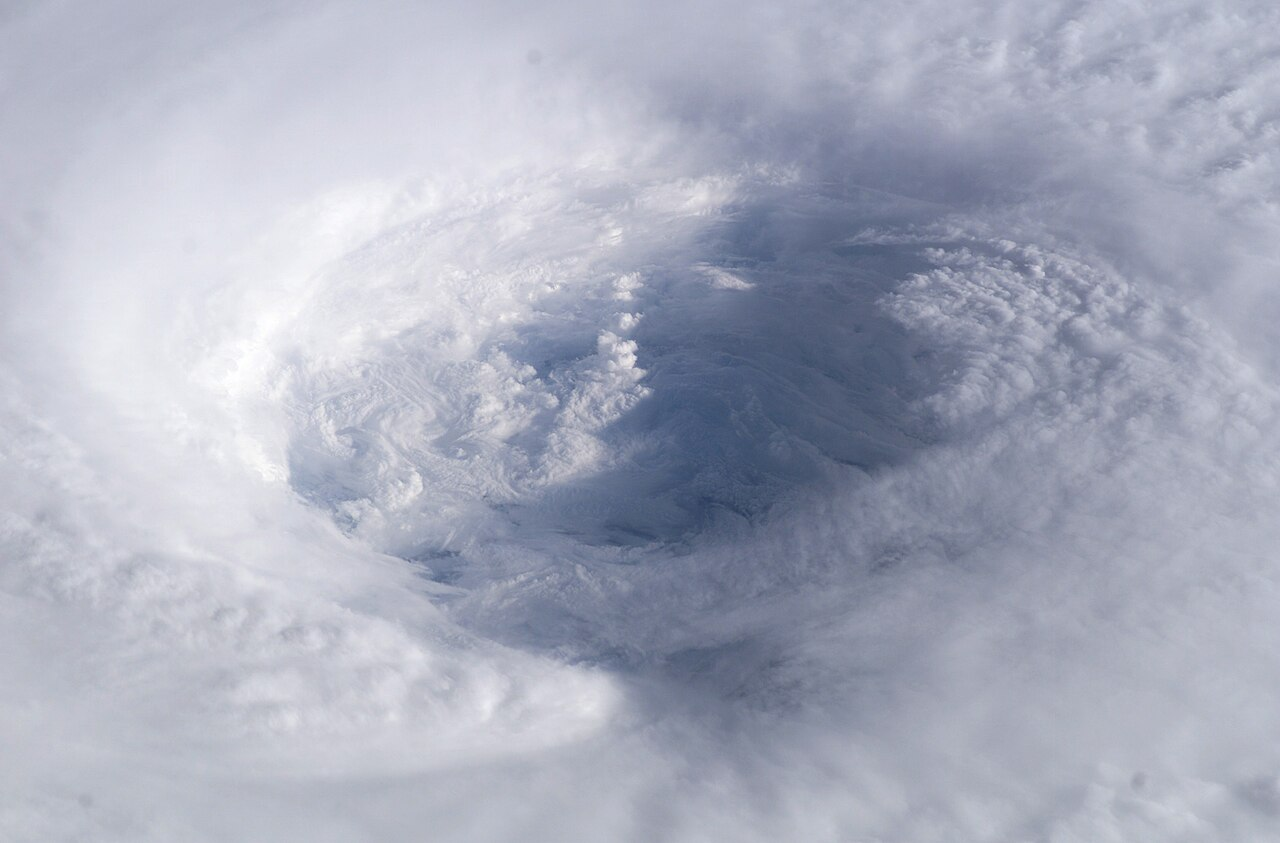
\includegraphics[width=0.5\linewidth]{images/book1/g5-hurricane-isabel-iss.jpg}

{\small 从国际空间站向下俯瞰 2003 年 9 月大西洋上空飓风“伊莎贝尔”的
\omterm{def:g5:natural-hazards:storm}{风暴}眼，一道云墙环绕着较为平静的中心。
照片：NASA，公有领域。}
% ledger: nasa:isabel-iss
\end{omfigure}

有些来自空气的危害进展缓慢、悄无声息。\emph{热浪}是指
连续数天、夜晚都比平常热得多的一段时期。它
对年老的人、婴儿和病人尤其危险。

\begin{definition}[干旱]\label{def:g5:natural-hazards:drought}
\emph{干旱}\index{干旱}是指持续数月甚至数年、
降雨量远低于该地区平常水平的一段较长时期。土壤变干，\omterm{def:g1:landscapes-around-us:water}{河流}
和\omterm{def:g1:landscapes-around-us:water}{湖泊}萎缩，庄稼枯萎死亡。
\end{definition}

\omterm{def:g5:natural-hazards:drought}{干旱}是慢慢来临的，没有人能说出它究竟从哪一天开始。但
长时间的\omterm{def:g5:natural-hazards:drought}{干旱}可能使农民颗粒无收，使城镇缺水。

\begin{omfigure}
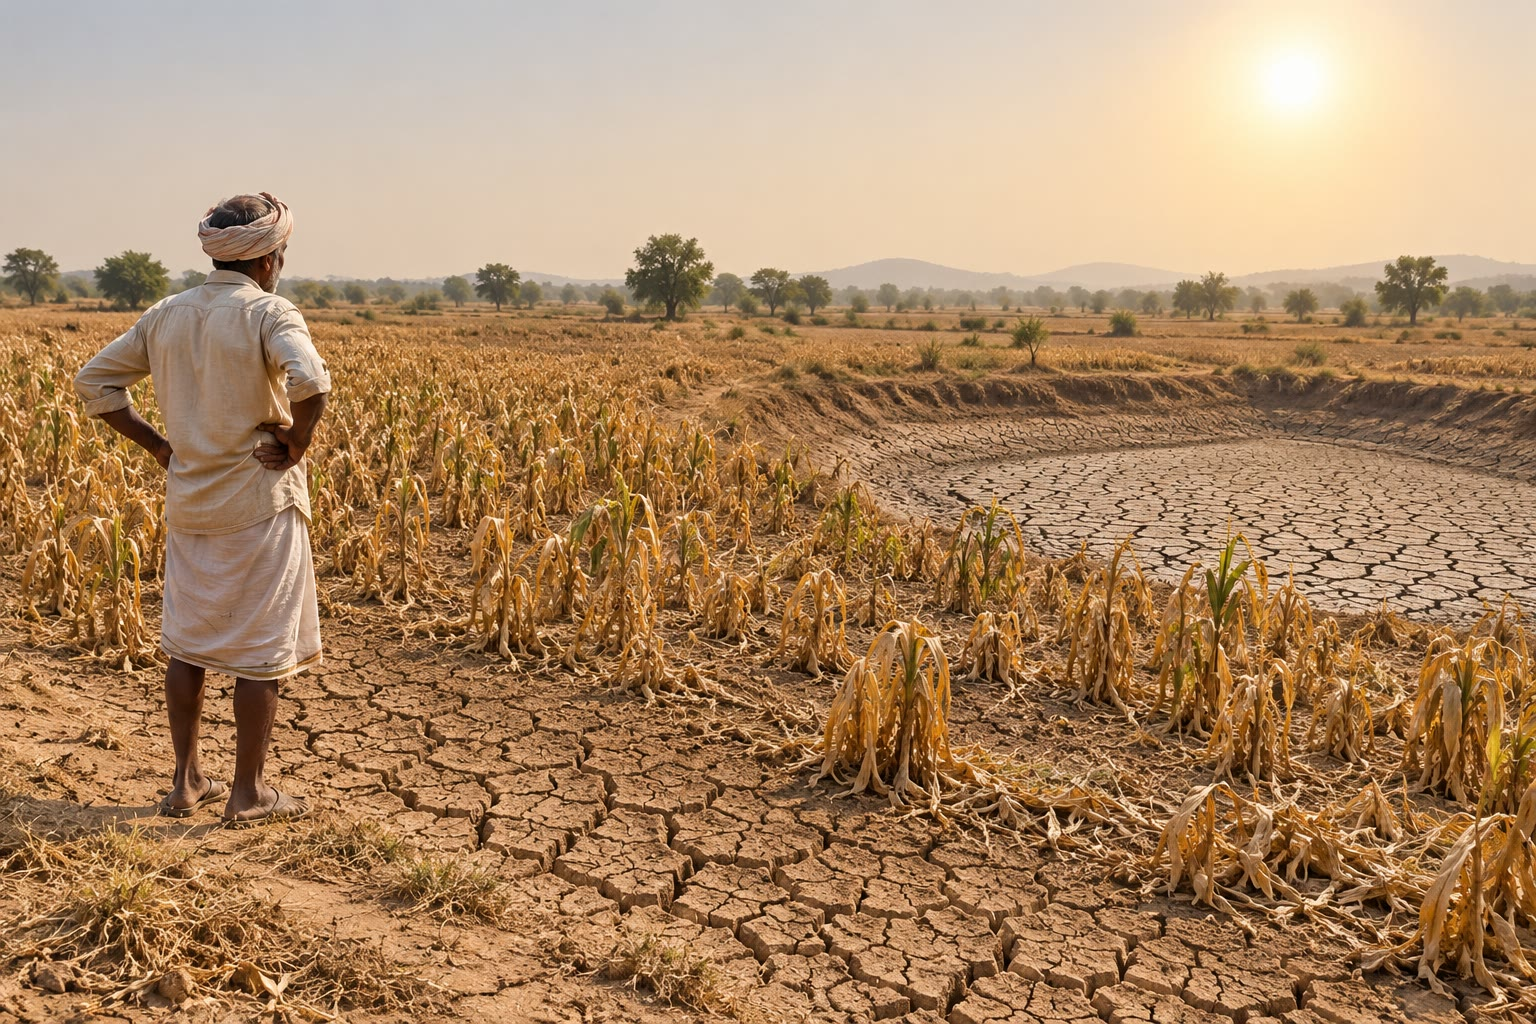
\includegraphics[width=0.42\linewidth]{images/book1/ai/g5-drought-field.jpg}

{\small 长期\omterm{def:g5:natural-hazards:drought}{干旱}中的田地：土地龟裂，庄稼发黄，
池塘已经干涸。}
\end{omfigure}

\section{水带来的危害}

你已经知道\omterm{def:g1:landscapes-around-us:water}{河流}的\omterm{def:g5:water-shapes-the-land:flood}{洪水}（见\cref{ch:g5:water-shapes-the-land}）。
连续数日降雨，或雪融化得很快时，河水
会涨过河岸，淹没\omterm{def:g5:water-shapes-the-land:flood}{河漫滩}。有些\omterm{def:g5:water-shapes-the-land:flood}{洪水}来得非常快：一场猛烈的暴雨
落在陡峭的\omterm{def:g1:landscapes-around-us:landform}{山谷}上，一小时内就能把平静的小溪变成咆哮的急流。
另一些\omterm{def:g5:water-shapes-the-land:flood}{洪水}来自\omterm{def:g2:water-on-earth:ocean}{海洋}：\omterm{def:g5:natural-hazards:storm}{风暴}把海水推上
低矮的\omterm{def:g1:landscapes-around-us:water}{海岸}。

\section{来自地面的危害}

你已经知道\omterm{def:g4:volcanoes-earthquakes-first-look:earthquake}{地震}和\omterm{def:g4:volcanoes-earthquakes-first-look:volcano}{火山}\omterm{def:g4:volcanoes-earthquakes-first-look:eruption}{喷发}
（见\cref{ch:g4:volcanoes-earthquakes-first-look}）。还有第三种来自地面的危害，
而且水常常会引发它。

\begin{definition}[滑坡]\label{def:g5:natural-hazards:landslide}
\emph{滑坡}\index{滑坡}是指\omterm{def:g3:stones-pebbles-sand:rock}{岩石}、土壤或泥土组成的
块体突然沿斜坡滑动或坠落。
\end{definition}

陡坡在长时间降雨浸泡下变得又重又滑，
可能会一下子整体滑落。\omterm{def:g4:volcanoes-earthquakes-first-look:earthquake}{地震}也能震松斜坡。\omterm{def:g5:natural-hazards:landslide}{滑坡}
可能掩埋道路、堵塞\omterm{def:g1:landscapes-around-us:water}{河流}，或把房屋冲走。

\begin{omfigure}
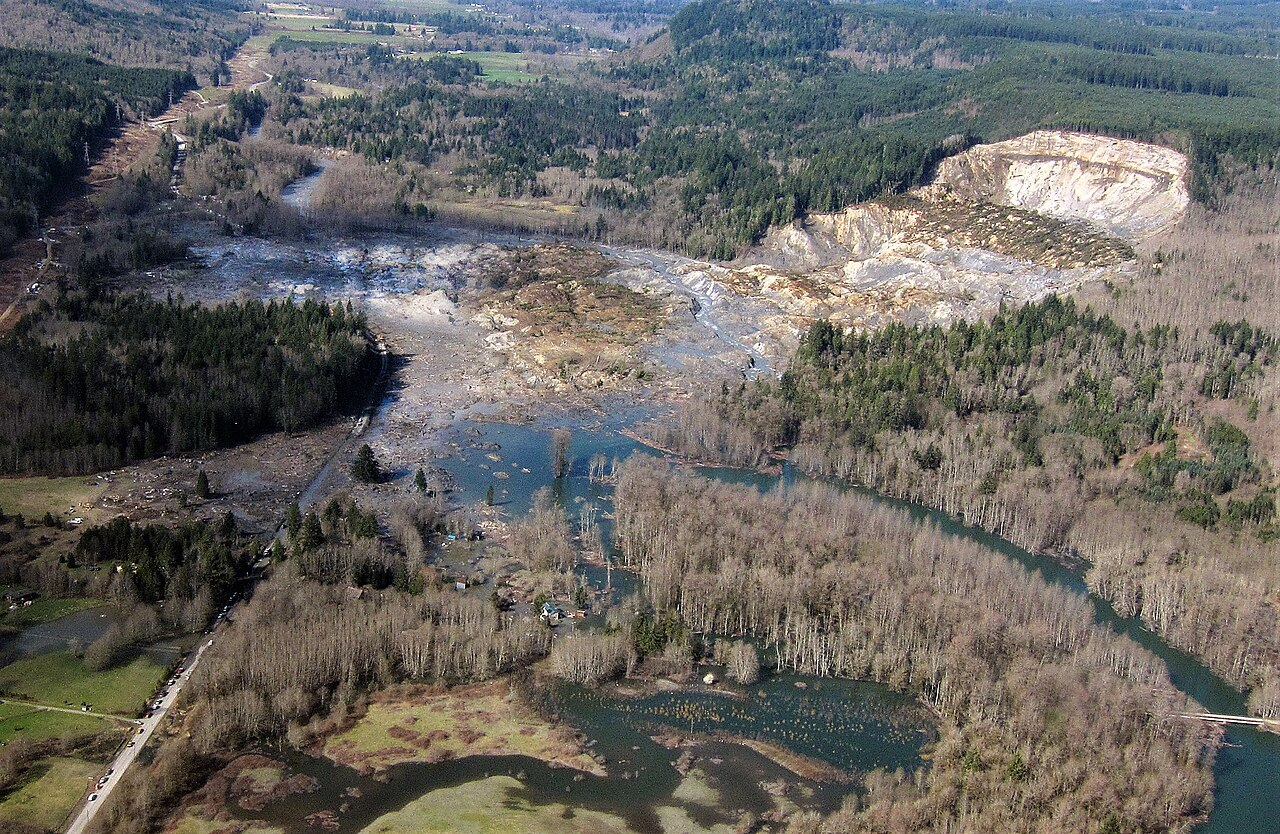
\includegraphics[width=0.6\linewidth]{images/book1/g5-landslide-washington.jpg}

{\small 2014 年美国华盛顿州发生的一次大型\omterm{def:g5:natural-hazards:landslide}{滑坡}，
从飞机上拍摄。右侧山坡已经崩塌，其泥土
铺满了整个\omterm{def:g1:landscapes-around-us:landform}{山谷}，掩埋了一条道路，并堵塞了\omterm{def:g1:landscapes-around-us:water}{河流}，
使上游的树林被淹没。照片：Mark Reid, U.S.
Geological Survey，公有领域。}\label{fig:g5:natural-hazards:landslide}
% ledger: usgs:oso-aerial
\end{omfigure}

\section{从危害到灾害}

开阔海面上的\omterm{def:g5:natural-hazards:storm}{风暴}、荒无人烟的\omterm{def:g5:weather-and-climate:desert}{沙漠}里的\omterm{def:g4:volcanoes-earthquakes-first-look:earthquake}{地震}、无人居住的\omterm{def:g1:landscapes-around-us:landform}{山谷}中的\omterm{def:g5:water-shapes-the-land:flood}{洪水}：
这些都是\omterm{def:g5:natural-hazards:hazard}{自然危害}，但它们不伤害任何人。
同样的事件一旦发生在人们居住的地方，就会变得危险。

\begin{definition}[自然灾害]\label{def:g5:natural-hazards:disaster}
\emph{自然灾害}\index{自然灾害}是指\omterm{def:g5:natural-hazards:hazard}{自然危害}袭击人们居住的地方，
并造成严重伤害：人员受伤或死亡，
房屋被毁，道路、供水和供电中断。
\end{definition}

\begin{omfigure}
\begin{tikzpicture}[x=1cm, y=1cm, font=\scriptsize]
  \foreach \dx/\title in {0/{空旷山谷中的洪水：\\一种自然危害},
                          7.6/{同样的洪水来到村庄：\\一场自然灾害}} {
    \begin{scope}[xshift=\dx cm]
      % valley sides
      \fill[green!25!brown!30] (0,0) -- (0,2.6) -- (0.4,2.6) -- (1.2,1.0) -- (5.6,1.0)
        -- (6.4,2.6) -- (6.8,2.6) -- (6.8,0) -- cycle;
      \draw[gray!60!black] (0,2.6) -- (0.4,2.6) -- (1.2,1.0) -- (5.6,1.0) -- (6.4,2.6) -- (6.8,2.6);
      % flood water over the whole valley floor
      \fill[blue!30, opacity=0.8] (1.05,1.2) -- (5.75,1.2) -- (5.6,1.0) -- (1.2,1.0) -- cycle;
      \fill[blue!30, opacity=0.8] (1.05,1.2) rectangle (5.75,1.5);
      \draw[blue!60!black] (0.95,1.5) -- (5.85,1.5);
      \node[align=center, anchor=north] at (3.4,-0.1) {\title};
    \end{scope}
  }
  % trees in the empty valley
  \foreach \x in {1.7,2.6,4.4,5.1} {
    \draw[brown!60!black, line width=1pt] (\x,1.0) -- (\x,1.75);
    \fill[green!50!black] (\x,1.95) circle (0.25);
  }
  % houses in the village valley
  \begin{scope}[xshift=7.6cm]
    \foreach \x in {1.6,2.5,3.4,4.3,5.1} {
      \fill[white, draw=black] (\x-0.3,1.0) rectangle (\x+0.3,1.65);
      \fill[red!60!black] (\x-0.38,1.65) -- (\x,2.0) -- (\x+0.38,1.65) -- cycle;
      \fill[blue!30, opacity=0.8] (\x-0.3,1.0) rectangle (\x+0.3,1.5);
    }
    % one house on the high ground, dry
    \fill[white, draw=black] (6.45,2.6) rectangle (6.77,2.95);
    \fill[red!60!black] (6.40,2.95) -- (6.61,3.2) -- (6.82,2.95) -- cycle;
  \end{scope}
\end{tikzpicture}

{\small 同一场\omterm{def:g5:water-shapes-the-land:flood}{洪水}，两种情形。在空旷的\omterm{def:g1:landscapes-around-us:landform}{山谷}中，它不伤害任何人；在
\omterm{def:g5:water-shapes-the-land:flood}{河漫滩}上建起村庄后，\omterm{def:g5:water-shapes-the-land:flood}{洪水}会灌入房屋。高处的房屋
依然保持干燥。}
\end{omfigure}

\omterm{def:g5:natural-hazards:storm}{风暴}和\omterm{def:g4:volcanoes-earthquakes-first-look:earthquake}{地震}无法阻止。但我们可以做很多事，
防止\omterm{def:g5:natural-hazards:hazard}{自然危害}演变为\omterm{def:g5:natural-hazards:disaster}{自然灾害}：不在\omterm{def:g5:water-shapes-the-land:flood}{河漫滩}和
不稳定斜坡的坡脚建房，把建筑修得坚固，留意\omterm{def:g1:watching-the-weather:weather}{天气}
和地面的变化，及时警告人们，并教会每个人应该怎么做。

\subsection*{预警}

气象部门日夜监测天空。当\omterm{def:g5:natural-hazards:storm}{风暴}、热浪或
\omterm{def:g5:water-shapes-the-land:flood}{洪水}即将来临时，他们通过广播、电视、电话和
互联网发出预警。许多国家用颜色表示预警级别，
从最平缓到最严重。

\begin{omfigure}
\begin{tikzpicture}[font=\small, wstep/.style={draw=black!60, minimum width=2.6cm,
    minimum height=0.8cm, font=\small\bfseries, rounded corners=2pt}]
  \node[wstep, fill=green!45] (g) at (0,0) {绿色};
  \node[wstep, fill=yellow!60] (y) at (0.6,0.95) {黄色};
  \node[wstep, fill=orange!70] (o) at (1.2,1.9) {橙色};
  \node[wstep, fill=red!65, text=white] (r) at (1.8,2.85) {红色};
  \node[anchor=west] at ($(g.east)+(0.3,0)$) {没有特别的危险};
  \node[anchor=west] at ($(y.east)+(0.3,0)$) {请当心，保持关注};
  \node[anchor=west] at ($(o.east)+(0.3,0)$) {做好准备：很可能有危险};
  \node[anchor=west] at ($(r.east)+(0.3,0)$) {危险极大：立即行动，遵照指示};
\end{tikzpicture}

{\small 预警颜色的阶梯。各国对其确切含义的规定
有所不同，请始终听从预警附带的
指示。}
\end{omfigure}

\begin{safety}
\textbf{暴风雨时。}待在室内，远离窗户。不要出门
张望，并远离可能倒下的树木，以及
倒落的电线。

\textbf{\omterm{def:g5:water-shapes-the-land:flood}{洪水}时。}转移到较高的地面或楼层上。切勿
步行、骑车或乘车穿过\omterm{def:g5:water-shapes-the-land:flood}{洪水}：湍急的水流
只需一点就足以把人冲倒，或把汽车冲走。

\textbf{热浪时。}经常喝水，在阴凉处或
凉爽的房间里度过最热的时段，并探望年长的邻居。

\textbf{\omterm{def:g4:volcanoes-earthquakes-first-look:earthquake}{地震}时。}趴下、掩护、抓牢
（见\cref{ch:g4:volcanoes-earthquakes-first-look}）。

\textbf{任何时候。}听从预警，并
立即按负责人员的指示行事。
\end{safety}

\section{练习}

\begin{exercise}[$\star$]\label{exo:g5:natural-hazards:1}
仅属于\omterm{def:g5:natural-hazards:hazard}{自然危害}，还是属于\omterm{def:g5:natural-hazards:disaster}{自然灾害}？
\begin{enumerate}
  \item[(a)] \omterm{def:g4:volcanoes-earthquakes-first-look:earthquake}{地震}使一片空无一人的\omterm{def:g5:weather-and-climate:desert}{沙漠}发生震动。
  \item[(b)] 一场\omterm{def:g5:natural-hazards:storm}{风暴}掀掉了镇上许多房屋的屋顶。
  \item[(c)] \omterm{def:g5:natural-hazards:landslide}{滑坡}坠入了一处无人居住的\omterm{def:g1:landscapes-around-us:landform}{山谷}。
  \item[(d)] \omterm{def:g1:landscapes-around-us:water}{河流}淹没了一个村庄，并使房屋灌满了水。
\end{enumerate}
\end{exercise}

\begin{exercise}[$\star$]\label{exo:g5:natural-hazards:2}
将下列危害分为三类（分别来自空中、来自水、来自
地面）：\omterm{def:g5:natural-hazards:landslide}{滑坡}、热浪、\omterm{def:g5:water-shapes-the-land:flood}{洪水}、\omterm{def:g4:volcanoes-earthquakes-first-look:volcano}{火山}\omterm{def:g4:volcanoes-earthquakes-first-look:eruption}{喷发}、\omterm{def:g5:natural-hazards:storm}{风暴}、
\omterm{def:g5:natural-hazards:drought}{干旱}、\omterm{def:g4:volcanoes-earthquakes-first-look:earthquake}{地震}。
\end{exercise}

\begin{exercise}[$\star$]\label{exo:g5:natural-hazards:3}
什么是\omterm{def:g5:natural-hazards:drought}{干旱}？请给出长期\omterm{def:g5:natural-hazards:drought}{干旱}伤害人类的两种方式。
\end{exercise}

\begin{exercise}[$\star$]\label{exo:g5:natural-hazards:4}
广播宣布今晚发布红色\omterm{def:g5:natural-hazards:storm}{风暴}预警。请给出
你的家人应当采取的三项行动。
\end{exercise}

\begin{exercise}[$\star$]\label{exo:g5:natural-hazards:5}
一场带有\omterm{def:g5:natural-hazards:storm}{风暴}眼的强烈旋转\omterm{def:g5:natural-hazards:storm}{风暴}在温暖的热带海面
上形成。若它袭击 (a) 北大西洋的佛罗里达\omterm{def:g1:landscapes-around-us:water}{海岸}；
(b) 西北太平洋的日本；(c) 印度洋上的印度\omterm{def:g1:landscapes-around-us:water}{海岸}，
则分别称为什么？
\end{exercise}

\begin{exercise}[$\star$]\label{exo:g5:natural-hazards:6}
将四种预警颜色按从最低到最严重的顺序排列。
处于最严重的等级时，你应当怎么做？
\end{exercise}

\begin{exercise}[$\star\star$]\label{exo:g5:natural-hazards:7}
请观察位于
第~\pageref{fig:g5:natural-hazards:landslide}~页的\omterm{def:g5:natural-hazards:landslide}{滑坡}照片，描述\omterm{def:g5:natural-hazards:landslide}{滑坡}
对\omterm{def:g1:landscapes-around-us:landform}{山谷}造成了什么影响：山坡、道路和\omterm{def:g1:landscapes-around-us:water}{河流}各受到怎样的影响。
为什么上游的土地现在被水淹没了？
\end{exercise}

\begin{exercise}[$\star\star$]\label{exo:g5:natural-hazards:8}
汤姆说：“\omterm{def:g5:water-shapes-the-land:flood}{洪水}是自然现象，因此对它无能为力。”莉娜
说：“我们无法阻止\omterm{def:g1:landscapes-around-us:water}{河流}泛滥，但可以阻止\omterm{def:g5:water-shapes-the-land:flood}{洪水}
演变成灾难。”谁说得对？请用两个例子加以说明。
\end{exercise}

\begin{exercise}[$\star\star$]\label{exo:g5:natural-hazards:9}
在一个虚构的农业地区，通常每月降雨约
60 毫米。\omterm{def:g5:natural-hazards:drought}{干旱}期间，四个月中每个月的降雨量
只有平常的四分之一。
\begin{enumerate}
  \item[(a)] 通常四个月的降雨量是多少？
  \item[(b)] \omterm{def:g5:natural-hazards:drought}{干旱}期间，这四个月共降雨多少？
  \item[(c)] 缺少了多少降雨？
\end{enumerate}
\end{exercise}

\begin{exercise}[$\star\star$]\label{exo:g5:natural-hazards:10}
一个虚构的城镇有 1\,200 座房屋，其中四分之一
位于该河的\omterm{def:g5:water-shapes-the-land:flood}{河漫滩}上。
\begin{enumerate}
  \item[(a)] \omterm{def:g5:water-shapes-the-land:flood}{河漫滩}上有多少座房屋？
  \item[(b)] 镇上帮助其中三分之一房屋的业主迁往
        较高的地面。仍位于\omterm{def:g5:water-shapes-the-land:flood}{河漫滩}上的房屋有多少座？
\end{enumerate}
\end{exercise}

\begin{exercise}[$\star\star\star$]\label{exo:g5:natural-hazards:11}
两个相距遥远的村庄在同一夜遭遇了强度相同的
\omterm{def:g5:natural-hazards:storm}{风暴}。第一个村庄无人受伤，损失很小；第二个村庄
许多房屋被毁。请至少给出三条能解释这种差异的
不同原因。
\end{exercise}
